\chapter{Functioneel ontwerp SOUP API}\label{ch:impl soup api}
De SOUP-API is de centrale module voor het systeem dat verantwoordelijk is voor het periodiek scannen van de projecten, het parsen van de rapporten die uit de analyses komt en het beschikbaar maken van de data die in de datbase is opgeslagen. In dit hoofdstuk wordt functioneel ingegaan op de werking van dit deel van de applicatie en zijn de drie sub-modulen die ieders een deel van deze taken op zich neemt beschreven. Eerst zal de algmene functionaliteit van de API behandeld worden om vervolgens de iets grotere functies zoals het parsen van de SCA rapportage en het regelen van het periodieke analyse systeem te behandelen.


\section{API}\label{sec:api2}
Centraal in de SOUP-API staat de API welke verantwoordelijk is om de data die door de beide Engines, beschreven in het hoofdstuk Architectuur, te verwerken en in goede banen te leiden. De API zal de Controller, Service en Repository structuur aanhouden.

Om de data die in het datamodel (zie figuur~\ref{fig:SOUP-SoupApiDm [CHECKEN]} in het vorige hoofdstuk) gedefineerd is te bedienen is er gekozen voor een model, service , repository architectuur. voor iedere entiteit in het datamodel is een case class geschreven met daarbij een companionobject wat direct de mogelijkheid bied om deze classes om te zetten in JSON voor opslag in de database en verzenden van en naar de API. De business logica is belegt in services, waarbij er voor iedere entitiet een service is aangemaakt die mutaties op deze entiteiten mogelijk maakt. Waarbij naast de standaard CRUD acties ook relaties tussen de entiteiten kunnen worden gemaakt. De repository maakt het vervolgens mogelijk om data van en naar de database te versturen.

\begin{figure}[bth]
    \myfloatalign
    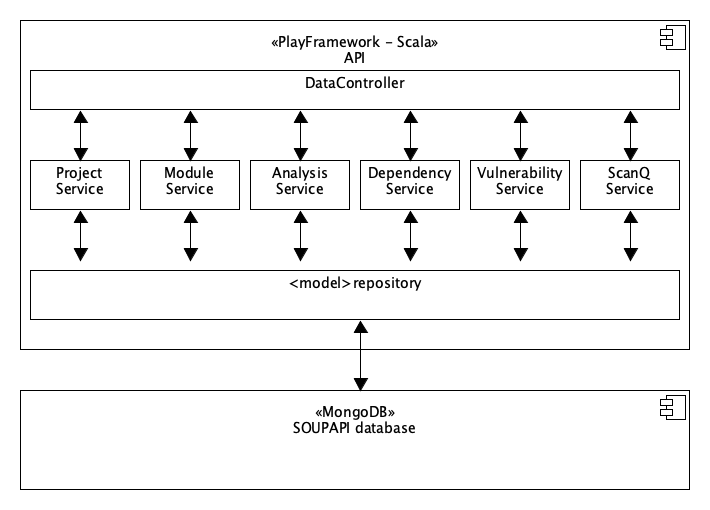
\includegraphics[width=12cm]{gfx/umlet/exports/API-ComponentsDiagram}
    \caption{API components Controllers , services en repositories}
    \label{fig:API components}
\end{figure}


\subsection{Controllers}\label{subsec:controllers}
Voor iedere entiteit dat belegt is in zowel het interne datamodel(figuur~\ref{fig:SOUP-SoupApiDm [CHECKEN]} als het datamodel voor de portal(figuur~\ref{fig:SOUP-portalDm})) worden algemene REST endpoints aangemaakt die bewerkingen op data beschikbaar maken waar dit gewenst en mogelijk is. Zo worden er waar nodig Create, Read, Update, Delete controllers aangemaakt.
\subsubsection{DataController}
Controller voor het beheer van de data in de database
\subsubsection*{Create}
Bij een create dient het ID van de aangemaakte entiteit te worden teruggeven aan de client
\textbf{POST: /data/[Entiteit]/} maakt een enititeit aan volgens de in de body meegegeven DTO die mee wordt gegeven.

\subsubsection*{Read}
Als er een read actie wordt aangeroepen kan alleen de entiteit op zichzelf worden weergegegeven of ook een gedetaileerde weergave.

\textbf{GET: /data/[Entiteit]/?detail=[boolean]} Haalt alle mogelijke records op van de betreffende entiteit. door detail op true te zetten komen ook alle sub entiteiten mee met de return body

\textbf{GET: /data/[Entiteit]/?detail="[boolean]"&attr="[attribuut]"&value="[value]} Haalt een enkele entiteit op van een enkel record op basis van het meegegeven attribuut en de value van dat attribuut. als er bijvoorbeeld een enkel project moet worden opgehaald op basis van de naam is de volgende HTTP POST Call op "/data/project/?detail=true&attr="name"&value="groeigids" de manier om het project groeigids op te halen.

\subsubsection*{Update}
\textbf{PUT: /data/[Entiteit]/?attr="[Attribuut]&value="[value]"} update een door de attribute en value geselecteerde record met de meegegeven body
\subsubsection*{Delete}
\textbf{DELETE: /data/[Entitiet]/?attr="[Attribuut]&value="[value]"} verwijderd een record dat gevonden wordt middels de meegegeven attribuut en de bijbehorende value

\subsubsection{UploadController}
De controller fungeerd als gateway waar rapporten naar kunnen worden geupload. Er kunnen vanuit twee processen binnen de SOUP applicatie rapporten worden geupload. Voor beide is een eigen endpoint voorzien:

\textbf{POST: /upload/jenkins} geeft een endpoint met de mogelijkheid om meerdere bestanden te uploaden. Als eerste is er het SCA rapport met daarin de resultaten van de eerste analyse. Bij de analyse middels jenkins worden ook de dependency files meegezonden om op die manier het systeem up-to-date te houden. Als laatst wordt er een JSON bestand meegestuurt met daarin de meta gegevens over het project.

\begin{figure}[bth]
    \myfloatalign
    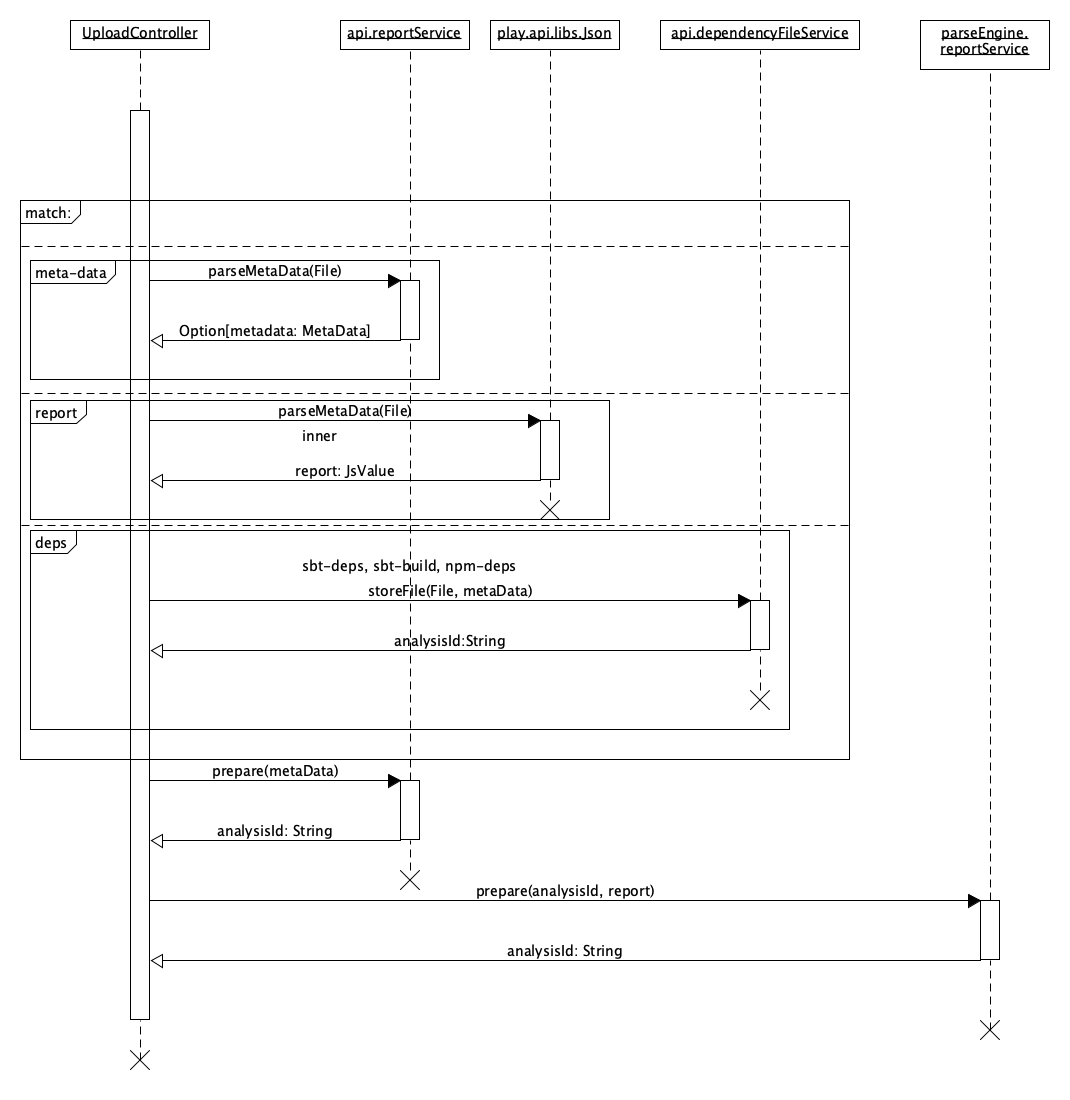
\includegraphics[width=12cm]{gfx/umlet/exports/SequploadController-Jenkins}
    \caption{Sequence UploadController Jenkins endpoint}
    \label{fig:SequenceUploadReportJenkins}
\end{figure}

\textbf{POST: /upload/pae} dit endpoint geeft alleen de mogelijkheid om het SCA rapport en de meta data up te loaden welke vervolgens worden verwerkt door de SOUPAPI. gezien er in de analysis engine geen veranderingen in de dependencies zijn hoeven deze dan ook niet worden meegezonden.

\begin{figure}[bth]
    \myfloatalign
    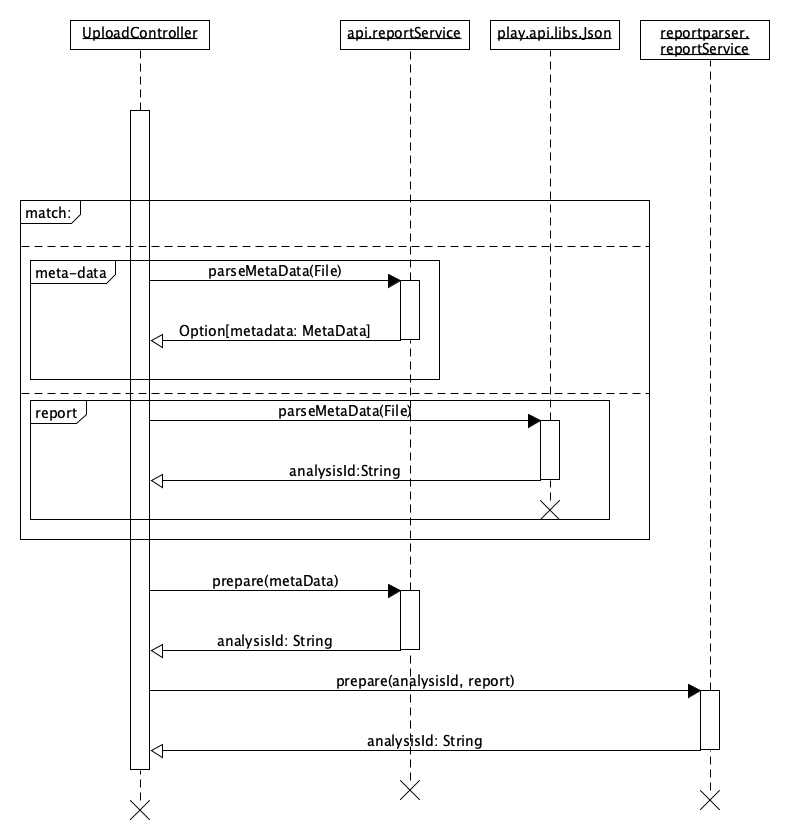
\includegraphics[width=12cm]{gfx/umlet/exports/SequploadController-pae}
    \caption{Sequence UploadController Periodic Analysis Engine endpoint}
    \label{fig:SequenceUploadReportpaet}
\end{figure}
In beide gevallen worden er bestanden naar de uploadcontroller verstuurt. Echter worden alleen dependencybestanden verstuurt naar de \texttt{/upload/jenkins/} endpoint. De bestanden zijn onderdeel van de body en worden voorzien van een key. Hieronder is te zien welke bestanden de controller kan verwachten en met welke key deze geidentificeert kan worden.

\begin{tabular}{lll}
    \textbf{key} & Type & \textbf{bestand} \\
    report & JSON & het SCA Rapport \\
    meta-data & JSON & Meta Data over de analyse uit jenkins \\
    sbt-deps & scala source & dependencydeclarite uit SBT project \\
    sbt-build & build.sbt  & build file van SBT project\\
    npm-deps & JSON & package-lock.json \\
\end{tabular} \\

Direct bij de controller worden de binnenkomende bestanden verwerkt de dependency bestanden worden middels een service opgeslagen in de fileSystem, de metaData wordt omgezet in een object van de case class MetaData zodat de attributen makkelijk te bereiken zijn. Het rapport wordt omgezet naar JSON zodat deze door de ReportParseEngine kan worden verwerkt.

\subsection{Services}\label{subsec:Services}
Voor de business logica is er een services laag die de verschillende processen in de SOAP-API belegt. In principe zijn er hoofd typen processen: De verwerking van rapportage over kwetsbaarheden en services die de bewerkingen op data regelen.
De Data services zijn een tussen laag tussen de dataControllers en de Datarepositories die het mogelijk maken om enititeiten toe te voegen en relaties tussen entiteiten te leggen. Het maakt het ook mogelijk om records op te halen op basis van deze relaties.

Daarnaast is er een reportservice die zorg draagt voor de communicatie van en naar de ReportParseEngine.



\subsection{Repositories}\label{subsec:repositories}
Net als bij de services is voor iedere Entiteit in het datamodel een eigen repository geschreven die de interactie met de database mogelijk maakt. In elke repository zijn de basis bewerkingen belegt. Dus voor iedere entiteit zijn onderstaande functies geschreven:

\begin{tabular}{ll}
    \textbf{function} & \textbf{Returns}\\
    create(e: Entity) & Future[Boolean] \\
    createMany(deps: Seq[Entity])& Future[Boolean]\\
    findOneById(id: String) & Future[Option[Entity]]\\
    findOneByName(name: String) & Future[Option[Entity]]\\
    findAll() & Future[Seq[Entity]] \\
    update(id: String, e: Entity) & Future[Boolean]\\
    delete(id: String) & Future[Boolean] \\
\end{tabular} \\

Naast de bovengenoemde functies zullen er voor een enkele repository nog extra functies moeten worden aangemaakt die hieronder genoemd zijn:

\begin{tabular}{lll}
    \textbf{Entiteit} & \textbf{function} & \textbf{Returns}\\
    enititeit & create(e: Entity) & Future[Boolean] \\
    enititeit & createMany(deps: Seq[Entity])& Future[Boolean]\\
    enititeit & findOneById(id: String) & Future[Option[Entity]]\\
    enititeit & findOneByName(name: String) & Future[Option[Entity]]\\
    enititeit & findAll() & Future[Seq[Entity]] \\
    enititeit & update(id: String, e: Entity) & Future[Boolean]\\
    enititeit & delete(id: String) & Future[Boolean] \\
\end{tabular} \\



%https://stackoverflow.com/questions/70513344/scala-generic-repository-class-for-reactive-mongo-repositoryalpakka-needed-c

\subsubsection{DTO's}
Omdat niet altijd het gehele object van en naar de client wordt verstuurt worden er DTO's aangemaakt. Deze kunnen worden gebruikt als afspraak tussen de backend en de client. Een voorbeeld van een DTO is de volgende:

In de jenkins upload controller wordt er naast een rapport ook metadata verstuurt middels een json bestand. In de backend is de volgende case class gedifineerd met de genodigde gegevens:
\begin{lstlisting}[caption={case class MetaData in MetaData.scala},label=lst:metdataScala]

package domain.dtos
import play.api.libs.json.{Json, OFormat}

case class MetaData(
                     projectName: String,
                     moduleName: String,
                     platform: String,
                     runtimeVersion: String,
                     buildToolVersion: String,
                     tool: String,
                     gitHash: String,
                     jenkinsBuildNr: String
                   )

object MetaData {

  implicit val projectFormat: OFormat[MetaData] = Json.format[MetaData]
}

\end{lstlisting}
Wat vervolgens in de volgende JSON resulteert:
\begin{lstlisting}[caption={metadata JSon object behorende bij de case class}, label={lst:metadatajson}]
{
  "projectName": "testProject",
  "moduleName": "backend",
  "platform": "sbt",
  "runtimeVersion": "2.13.6",
  "buildToolVersion": "1.5.0",
  "tool": "owasp",
  "gitHash": "6cf71dd74241e6292db69368f1d4f6d990b3f03s",
  "jenkinsBuildNr": "42"
}
\end{lstlisting}

\subsection{Algehele CRUD functionaliteit}\label{subsec:algehele-crud-functionaliteit}
sequence diagrammen voor:
\subsubsection*{Create}Schema maken
\subsubsection*{FindOne}Schema maken
\subsubsection*{FindAll}Schema maken
\subsubsection*{Update}Schema maken
\subsubsection*{Delete}Schema maken

\subsection{Toevoegen van entiteit A aan entiteit B}\label{subsec:toevoegen-van-entiteit-a-aan-entiteit-b}
Toevoegen van module aan project



\section{Report Parse Engine}
De ReportParseEngine is verantwoordelijk voor het omzetten van een rapport dat gegenereerd wordt door een Software Composition Analysis Tool naar het interne datamodel. Het feit dat er veel tools zijn die allemaal de mogelijkheid bieden om projecten te analyseren op kwetsbaarheden en hier een rapport over uit te brengen geeft al aan dat de ReportParseEngine in staat moet zijn om met verschillende rapporten van verschillende tools om moet kunnen gaan. Om dit te mogelijk te maken is er gekozen voor een modulaire opzet waarbij er verschillende parsers geschreven kunnen worden die de rapporten kunnen omzetten. Deze Modulaire opzet is te zien in figuur~\ref{fig:ReportParserComponents} waarbij de $"$[FUTURE]Parser$"$ een placeholder is voor elke parser die in de toekomst moet worden toegevoegd om meerdere tools te kunnen ondersteunen.
\begin{figure}[bth]
    \myfloatalign
    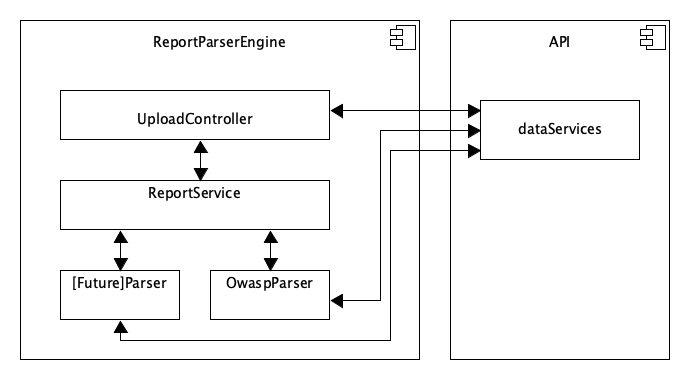
\includegraphics[width=12cm]{gfx/umlet/exports/ReportParserComponents}
    \caption{ReportParserEngine Components}
    \label{fig:ReportParserComponents}
\end{figure}


\subsection{ReportService}\label{subsec:reportservice}


In deze reportService zijn een aantal functies geimplementeerd die ervoor zorgdragen dat een binnenkomen rapport in JSON wordt weggeschreven in de database.
\begin{itemize}
    \item aanmaken van analyses zie figuur(~\ref{fig:analysisPrepare})
    \item selecteren van de juiste reportParser op basis van binnengekomen parameter"tool" zie figuur(~\ref{fig:selectReportParser})
    \item selecteren van het juiste path voor elk proces
\end{itemize}



\begin{figure}[bth]
    \myfloatalign
    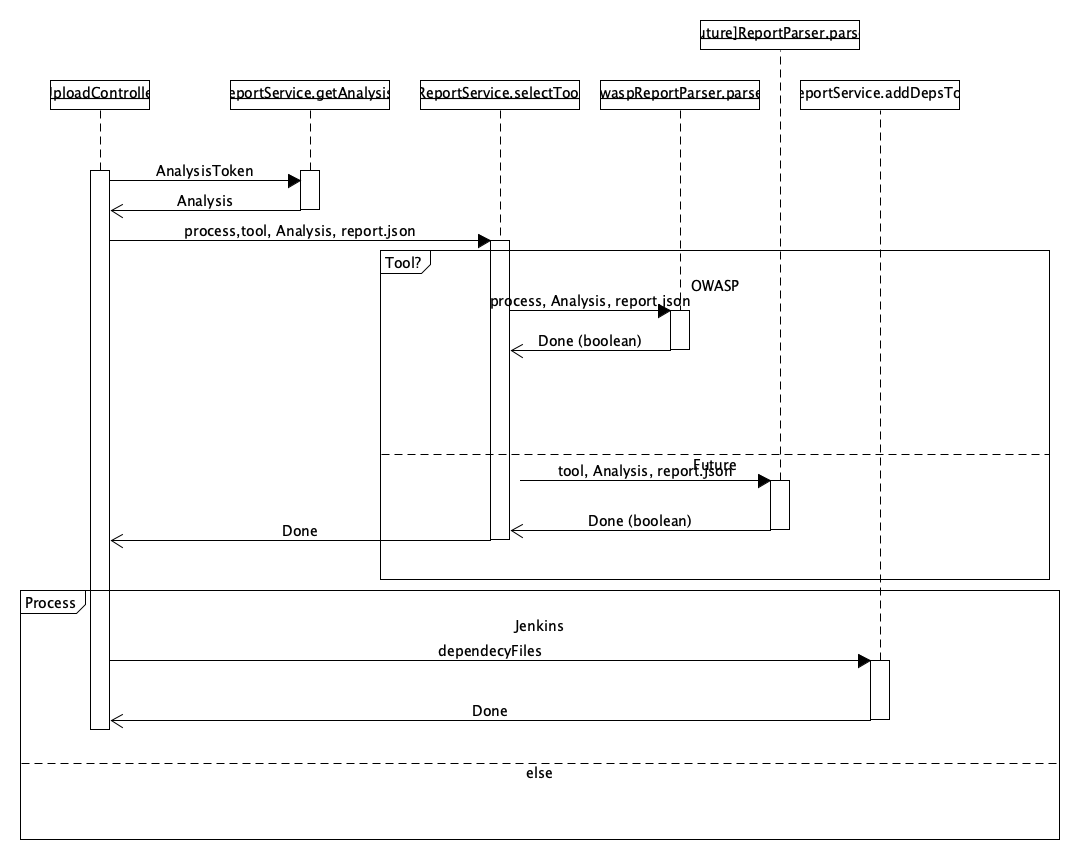
\includegraphics[width=14cm]{gfx/umlet/exports/SeqProcessPayload}
    \caption{Sequence diagram prepare Analysis}
    \label{fig:analysisPrepare}
\end{figure}

In het ontwerp is vastgelegt dat er altijd de mogleijkheid moet bestaan dat er tools toegevoegd kunnen worden aan de SOAP API. door dit mechanisme is dit mogelijk. Daarnasat moet er op het moment dat Jenkins de payload aanbied ook de dependencydeclaraties worden opgeslagen in de analyse.

\begin{figure}[bth]
    \myfloatalign
    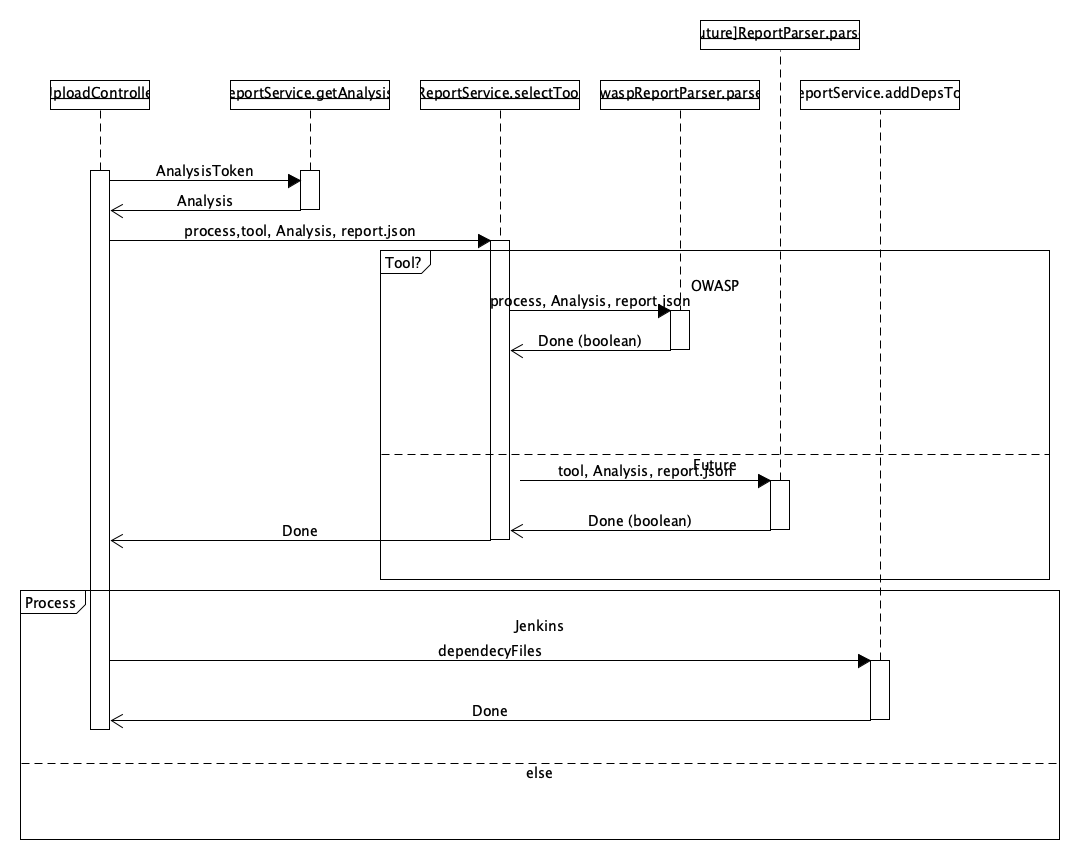
\includegraphics[width=14cm]{gfx/umlet/exports/SeqProcessPayload}
    \caption{Sequence diagram Proces Payload}
    \label{fig:ProcesPayload}
\end{figure}

\subsection{OWASP Parser}\label{subsec:owasp-parser}
De OWASP parser is verantwoordelijk voor het omzetten van binnengekomen OWASP data in JSON naar data in de database waarbij de relaties tot elkaar blijven bestaan.
Omdat in een eerdere stap er al een analyse is aangemaakt dient alleen nog de dependencies en de bijbehorende vulnerabilities te worden tegevoegd.

Zoals eerder benoemd is de OWASP parser verantwoordelijk voor het inlezen van een aangeboden JSON en deze vervolgens op te slaan in een database op basis van het interne datamodel. Om dit te bewerkstelligen dienen de volgende stappen te worden genomen:
Als eerst wordt er gekeken of het in de parameters meegegeven project bestaat binnen de SOUPAPI. Als dit het geval is dan wordt er gekeken of de meegegeven module in het project bestaat. Mocht het project niet bestaan dan wordt er één aangemaakt samen met de meegegeven module en de default SOAPAPI projectsettings. Mocht de module niet bestaan dan wordt deze aangemaakt met de parameters die meegegeven zijn en vervolgens toegevoegd aan het project.
Op het moment dat zowel het project als de module bestaan wordt er een analyse aangemaakt en toegevoegd aan de
module. Als het een upload is vanuit het JenkinsProces worden de meegezonden dependency declaraties opgeslagen. Daarnaast wordt er voor iedere dependency in het rapport bekeken of deze al in de database staat. Als dit het geval is dan wordt deze toegevoegd aan de analyse. Als de dependency nog niet bestaat wordt deze opgeslagen in de database en vervolgens toegevoegd aan de analyse. Vervolgens wordt de vulnerability toegevoegd en gelinkt aan de dependencies. en ook hier geld als de vulnerability al bestaat is er alleen een link nodig.
Als laatst wordt er een nieuwe analyse toegevoegd aan de scanQ waarna er een result HTTP 200/201 komt.
\begin{figure}[H]
    \myfloatalign
    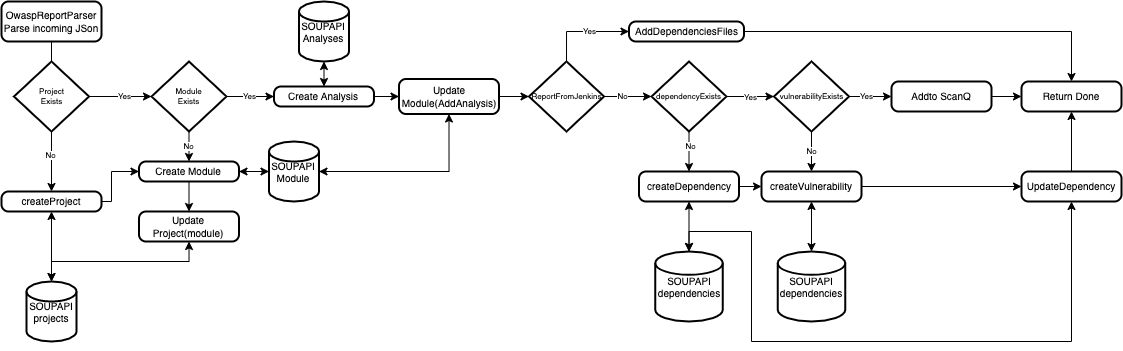
\includegraphics[width=15cm]{gfx/SOUPAPI-ReportParseFlow}
    \caption{Owasp Report Flow}
    \label{fig:OwaspReportFlow}
\end{figure}


\subsection{$"$[Future]Parser$"$}\label{subsec:$"$[future]parser$"$}
De $"$[Future]Parser$"$ zal in basis gelijk zijn als de parser voor de OWASP tool die hierboven worden beschreven. Echter zal de daadwerklijke omzetting veranderen. Om deze reden moet er voor iedere tool een eigen datamodel worden gedifineerd waarmee er objecten kunnen worden gemaakt van deze Data. Waarbij er vervolgens middels deze objecten naar het interne datamodel worden gewerkt.

\section{Periodiek Analysis Engine}

\subsection{ScanQ}
De ScanQ is een lijst waarin alle analyses in geplanned staan. Bij deze lijst zijn een aantal functies de lijst beheren.

De datastructuur van de lijst is als volgt:
\begin{itemize}
    \item projectnaam: Naam van het project
    \item lastAnalyses: timestamp van de laatste analyse
    \item nestAnalyses: timestamp voor de volgende analyse
\end{itemize}
De Controller is verantwoordelijk voor de taken die te maken hebben met het periodiek scannen van projecten Het heeft faciliteiten zoals een scanQ waarin de projecten staan die gescanned moeten worden. Een analyser die op het moment dat een project aan de beurt is om geanalyseerd te worden een aantal subtaken sequentieel uitvert per module binnen een project.
In grote lijnen wordt er een dockercontainer opgezet per module waarin alle benodigde bestanden (dependency declaraties en dergelijke) worden geplaats. Vervolgens een analyse wordt uitgevoerf waaruit de resultaten naar de ReportParser kan worden gestuurt voor analyse. De exacte werking wpordt verderop in het document technisch uitgewerkt.



\subsection{AnalysesController}\label{subsec:controller}
Naast de analyses die van de rapporten die uit het jenkins process komen is er ook behoefte om periodiek te analyseren op oudere niet actieve projecten. Om dit te kunnen faciliteren omnvat de Analyses controller een aantal componenten die ieders verantwoordelijk zijn voor een eigen taak:

\begin{figure}[H]
    \myfloatalign
    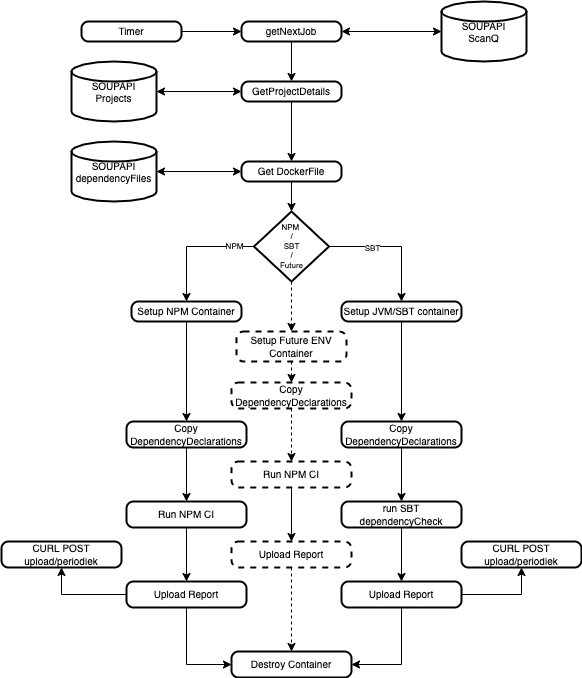
\includegraphics[width=10cm]{gfx/SOUPAPI-Periodic Analysis}
    \caption{Periodieke analyse flow}
    \label{fig:PeriodicAnalysis}
\end{figure}

\subsubsection{Timer}
De timer is verantwoordelijk voor het op tijd starten van de periodieke analyses op projecten die in de ScanQ staan. Op het moment dat er een geplannde analyse uitgevoerd moet worden zal deze aan de analyses controller worden gegeven die de verantwoordelijkheid overneemt.
\subsubsection{ScanQ + ScanQController}
De scanQ is een datastructuur gebasseerd op een list/seq waarin de analyses opgeslagen zijn die uitgevoerd moeten worden. De ScanQcontroller regelt de mutaties op deze scanQ.
\subsubsection{AnalysesController}
De analyse controller dient de taken uit te voeren die in figuur(~\ref{fig:PeriodicAnalysis}) weergegeven zijn. Dit is een sequenteel proces waarbij de controller wacht op antwoord voordat het een volgend onderdeel begint.

